\documentclass[a4paper,11pt]{article}
\usepackage{commonpackages}

\begin{document}
\title{Équations du deuxième degré}
\date{}
\maketitle


\section{Théorie}
L'expression sous la racine $$\Delta= \mathbf{b^2-4ac}$$ est appelée le \textbf{discriminant} et détermine le nombre de solutions d'une équation quadratique:\\
$\begin{array}{|l | l |}
\hline
\Delta>0 & \text{L'équation a \textbf{deux solutions} réelles} \\
& \text{Le polynôme factorisé est de la forme:}  a(x - x_{1})(x - x_{2}) \\
\hline
\Delta=0 & \text{L'équation a \textbf{une solution} réelle (solution double)}\\
& \text{Le polynôme factorisé est de la forme:}  a(x - x_{1})^2\\
\hline
\Delta<0 & \text{L'équation \textbf{n'a pas de solution} réelle}\\
& \text{Le polynôme ne peut pas être factorisé.}\\
\hline
\end{array}$\par

\section{Images}
Du texte avec des images:\par
Soit le triangle rectangle ABC rectangle en C dont $c$ est l'hypoténuse, $a$ et $b$ sont les cathètes et $c_{1}$ et $c_{2}$ sont les segments qui vont du pied de la hauteur ($H$) aux sommets adjacents ($A$ et $B$).\par
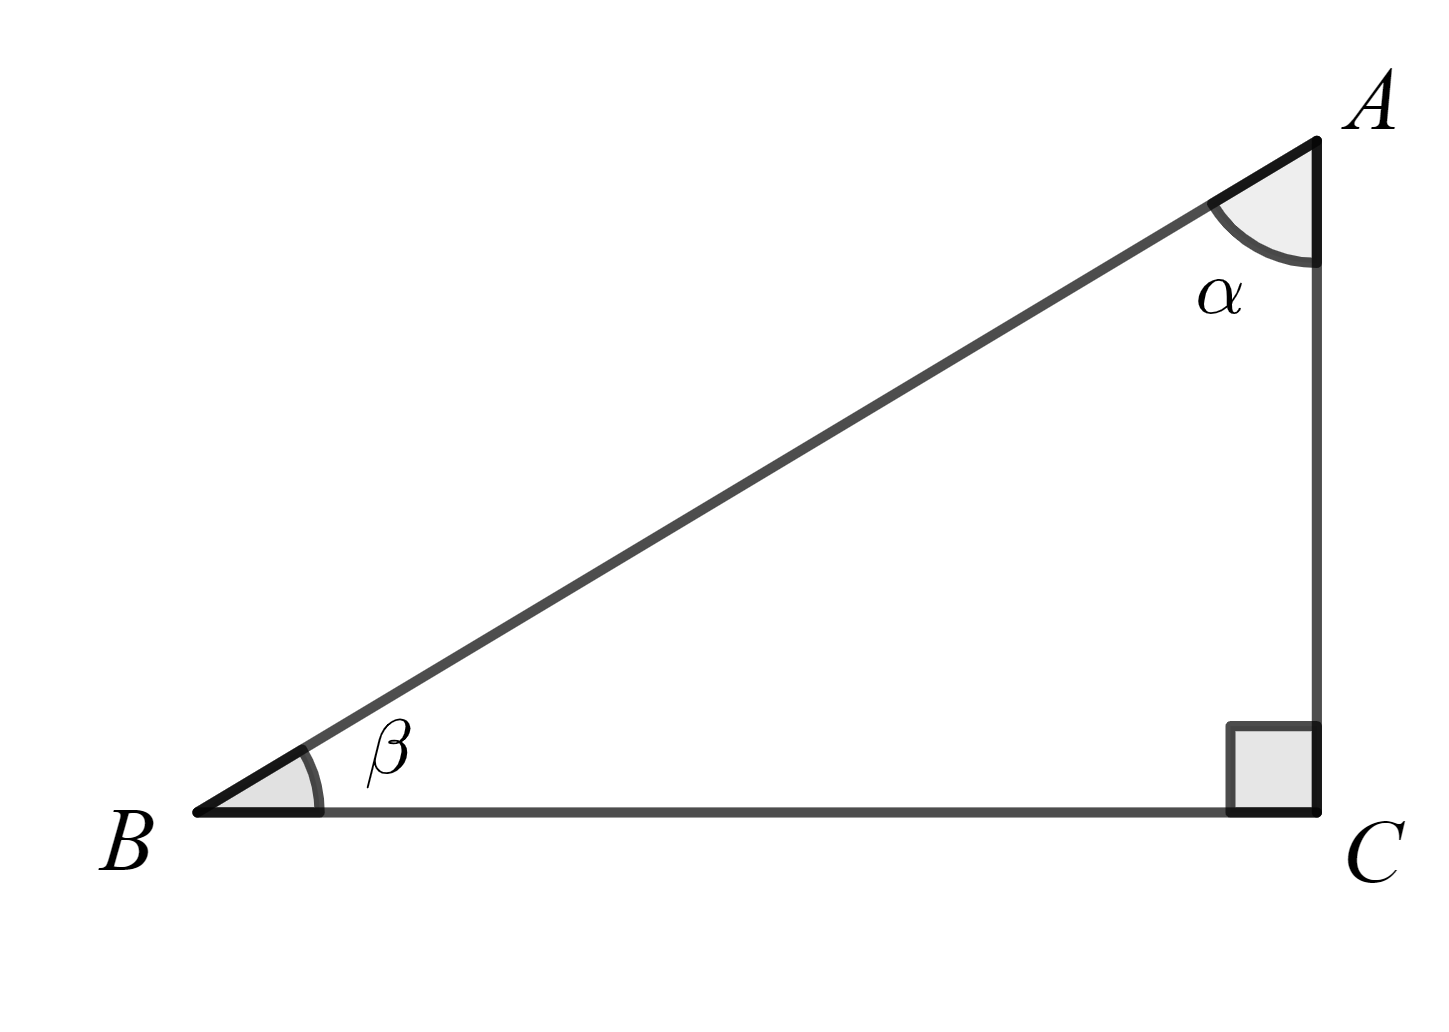
\includegraphics[width=0.3\textwidth]{images/pythagore.png}\\

\section{Vidéo}
Ici j'ajoute un lien vers une vidéo youtube:\par
\video{tc9wvbYuZts} %indiquer le pourcentage voulu par rapport à la largeur de la page

\section{Geogebra}
Ici j'ajoute un lien vers un document geogebra:\par
\geogebra[100]{cpmbrfxg} %indiquer le pourcentage voulu par rapport à la largeur de la page

\section{Python}
Ici j'ajoute du code python directement dans le document:\par
\begin{verbatim}{python}
for i in range(4):
    for j in range(5):
        print(i*j)
\end{verbatim}

\end{document}
